\chapter{Estado del arte}
En este capítulo se hablará sobre el contexto en el que se enmarca este proyecto.

En primer lugar, se hará una breve explicación de como las herramientas open-source ayudan a agilizar el desarrollo y la funcionalidad en una red de telecomunicaciones.

Por último, se hace especial mención a los dos paradigmas que motivan este proyecto: SDN y NFV.

\section{Herramientas Open-Source en redes de telecomunicación}

Una red de telecomunicación es un conjunto de medios, tecnologías y protocolos que tienen como finalidad el intercambio de información entre diferentes usuarios.

Así mismo, se está produciendo una enorme evolución en el concepto de una red de telecomunicación. 

Antes, este concepto era puramente físico, con un conjunto de dispositivos \textit{Hardware}, como pueden ser \textit{routers}, \textit{switches} u ordenadores, interactuando entre sí. Actualmente, prácticamente el 100\% de las redes utilizan software open-source para diferentes propósitos:

\begin{itemize}
	\item Sacar el máximo rendimiento a su infraestructura.
	\item Agilizar el envío y procesamiento del tráfico de la red.
	\item Acelerar y automatizar la gestión y configuración de los dispositivos.
	\item Reducir los costes de operación de la red.
\end{itemize}

Para conseguir los propósitos mencionados anteriormente, existen numerosas herramientas de software desarrolladas por empresas, universidades u organizaciones que están totalmente disponibles para ser usadas por cualquier usuario.

Dichas herramientas forman un gran conjunto heterogéneo, siendo desarrollada cada una de ellas para uno o más propósitos:

\begin{itemize}
	\item Para sacar el máximo rendimiento a la infraestructura de una red, existen herramientas de virtualización como \textbf{OpenStack} (ver \ref{sec:openstack}) o \textbf{Docker}, para proveer a las aplicaciones de una abstracción e independencia. Este tipo de herramientas pertenecen al paradigma \textbf{NFV} (ver \ref{sec:nfv}).
	
	\item Para agilizar el envío y procesamiento del tráfico de una red, existen herramientas que permiten crear dispositivos hardware virtualizados como \textbf{OpenVSwitch} o \textbf{Mininet} (ver \ref{sec:mininet}). Gracias a este tipo de herramientas, se puede sustituir un \textit{Switch} clásico por un pequeño software que hace las funciones de un \textit{Switch} de una manera más eficiente.
	
	\item La gestión de los dispositivos se ha realizado de forma manual, dispositivo a dispositivo. Gracias a herramientas software como \textbf{Cacti} o \textbf{Nagios}, la forma de gestionar las redes de telecomunicación ha dado un giro de 180 grados. Utilizando estas herramientas, el usuario puede gestionar la red desde un terminal de manera remota, gracias al protocolo SNMP (\textbf{Simple Network Management Protocol}).
	
	\item Para acelerar y automatizar la configuración de los dispositivos de una red de telecomunicación, existen herramientas que pertenecen al paradigma \textit{SDN} (ver \ref{sec:sdn}). Un ejemplo de estas herramientas es el controlador SDN ONOS (ver \ref{sec:onos}).
	
	\item Para reducir los costes de operación de una red, existen herramientas open-source que ayudan a planificar una red de telecomunicación de forma óptima. La más conocida de estas herramientas es \textbf{Net2Plan} (ver \ref{sec:net2plan}), una herramienta de planificación de redes programada en Java.
\end{itemize}

\section{SDN}
\label{sec:sdn}

SDN (\textit{Software Defined Networking}) es un paradigma que consiste en una nueva forma de configurar las redes de telecomunicación. Su principal premisa es la de separar el plano de control (\textit{Software}) del plano de datos (\textit{Hardware}).

SDN pretende cambiar la manera tradicional de configuración de dispositivos usando instrucciones de bajo nivel por una manera novedosa mediante herramientas software a un alto nivel.

SDN surge principalmente por las limitaciones que tienen las tecnologías de redes actualmente. Las dos principales limitaciones son:

\begin{itemize}
	\item \textbf{Dificultad de escalabilidad:} A medida que el tráfico de una red aumenta, la red debe hacer lo mismo. Esto implica nuevos aparatos que deben ser configurados y gestionados. La cantidad de aparatos de una red aumenta de forma exponencial, y ello las hace que la infraestructura de una red sea difícilmente sostenible en cuanto a la configuración y gestión tradicionales.
	
	\item \textbf{Dependencia del fabricante:} Cada fabricante diseña sus dispositivos de red de una manera particular, con su propio sistema operativo y su propia sintaxis de configuración. En una red de telecomunicaciones es habitual que su infraestructura de red esté compuesta por dispositivos de diferentes vendedores y fabricantes, y es necesario conocer a fondo cada uno de los sistemas operativos.
	
\end{itemize}

Una vez identificadas las limitaciones de redes actuales, hay que identificar los beneficios que SDN puede dar a las entidades que opten por esta tecnología en sus redes de telecomunicaciones. Los principales beneficios de SDN son:

\begin{itemize}
	\item \textbf{Reducción del CapEx (\textit{Capital Expenditures}):} CapEx son los costes asociados a bienes físicos. SDN reduce la necesidad de invertir en nuevos bienes físicos (\textit{hardware}), ya que, gracias a su naturaleza, mediante \textit{software} es capaz de reducir notablemente la carga de trabajo de los dispositivos.
	
	\item \textbf{Reducción del OpEx (\textit{Operational Expenditures}):} OpEx son los costes asociados a operaciones y servicios. SDN reduce este tipo de costes debido a su configuración y gestión de los elementos de red mediante \textit{software}. Este control se realiza de forma más sencilla y automática, lo que permite una reducción del tiempo empleado por los administradores de la red.
	
	\item \textbf{Agilidad y flexibilidad:} SDN permite a las diferentes entidades desplegar aplicaciones, servicios e infraestructuras de forma rápida para alcanzar objetivos en el menor tiempo posible.
\end{itemize}

\subsection{Arquitectura SDN}

Las redes definidas por \textit{software} constan de una arquitectura de red específica, compuesta por distintos componentes \textit{hardware} y \textit{software} que interactúan entre sí, como se puede ver en la figura \ref{fig:arquitecturasdn}.
 
\begin{figure}[!ht]
	\centering
	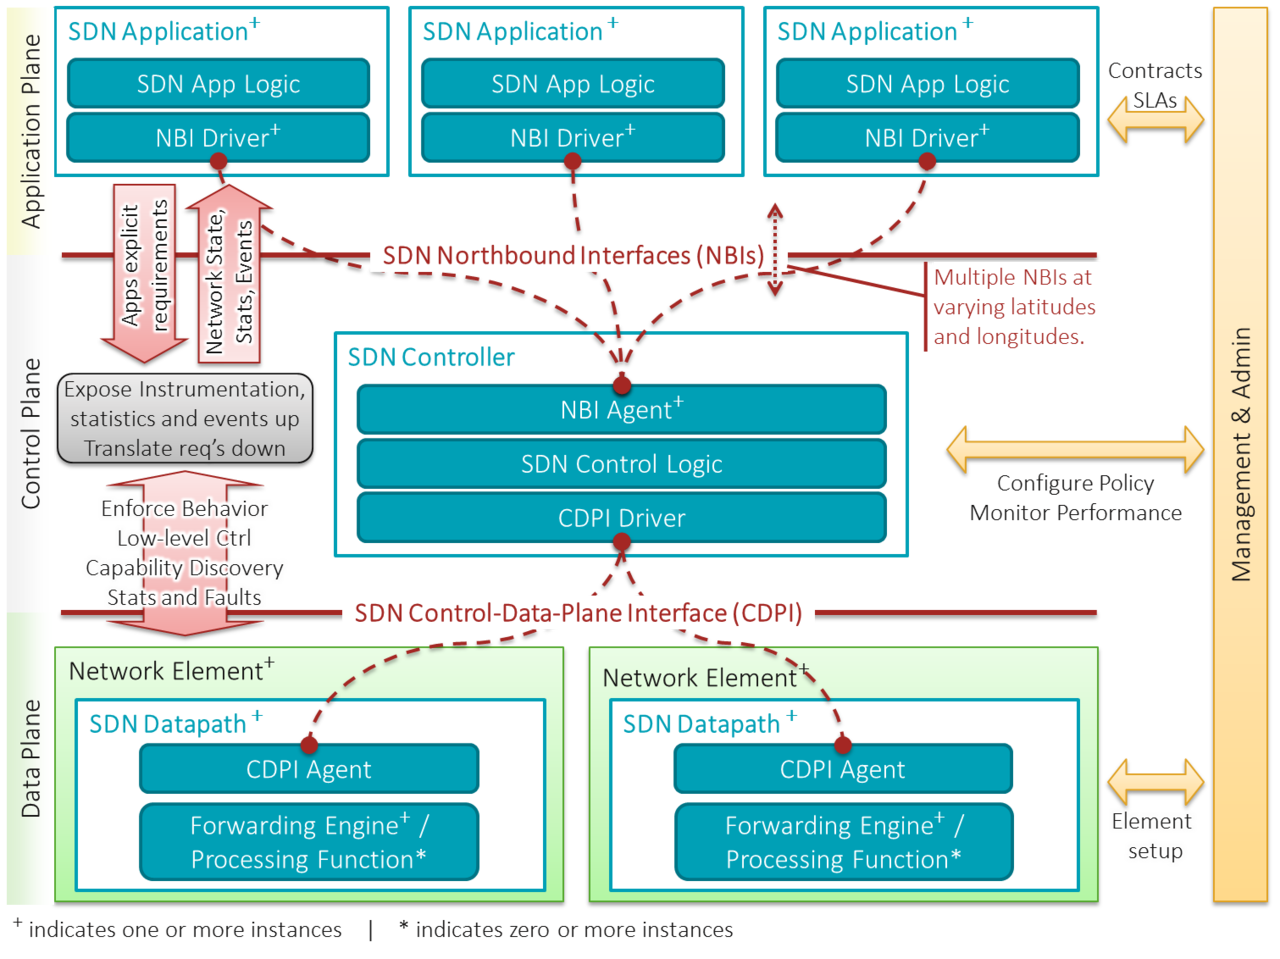
\includegraphics[width=0.75\linewidth]{imagenes/arquitectura_sdn}
	\caption{Arquitectura SDN  Fuente: https://es.wikipedia.org/wiki/Redes\_definidas\_por\_software}
	\label{fig:arquitecturasdn}
\end{figure}

Los diferentes elementos que componen la arquitectura SDN son los siguientes:

\begin{itemize}
	\item \textbf{Controlador SDN:} Es el cerebro de la red SDN. Forma el núcleo de la arquitectura SDN comunicándose con los \textit{switches} a través de la \textbf{Interfaz Sur} (\textit{SouthBound Interface}) y con las distintas aplicaciones a través de la \textbf{Interfaz Norte} (\textit{NorthBound Interface}).
	
	\item \textbf{Interfaz Sur:} Es la interfaz que conecta al controlador SDN con el plano de datos. Facilita la configuración de la red, transfiriendo dichas configuraciones a los dispositivos de la red. El protocolo más utilizado en esta interfaz es \textbf{OpenFlow} (ver \ref{subsec:openflow}).
	
	\item \textbf{Interfaz Norte:} Es la interfaz que conecta al controlador SDN con el plano de control. Facilita el proceso de automatización de la red mediante la comunicación del controlador con las diferentes aplicaciones. Para permitir dicha comunicación con las aplicaciones, la interfaz norte exporta una REST-API.
	
	\item \textbf{Agentes y \textit{Drivers}:} Para establecer la comunicación entre el controlador y los dispositivos mediante la interfaz sur y para la comunicación entre el controlador y las aplicaciones mediante la interfaz norte,es necesario un par agente-\textit{driver}. El \textit{driver} se encuentra en el controlador, mientras que el agente se encuentra en el dispositivo. Se encargan de realizar la comunicación en el plano de datos, realizando la conversión del lenguaje del controlador al del dispositivo, y viceversa.
	
	\item \textbf{Aplicaciones SDN:} Son programas que se conectan al controlador SDN mediante la interfaz norte. Gracias a su lógica de aplicaciones, desarrollan un próposito concreto y transfieren datos u órdenes al controlador SDN.
\end{itemize}


\subsection{OpenFlow}
\label{subsec:openflow}

OpenFlow es un protocolo estándar de SDN, siendo el más utilizado para comunicar el controlador SDN con los dispositivos que se encuentran en el plano de datos. Para que esta comunicación sea posible, el controlador SDN debe tener operando un driver OpenFlow, mientras que el dispositivo debe tener corriendo un agente OpenFlow. 

Un \textit{switch} tradicional utiliza su propia lógica de encaminamiento para decidir como tiene que reenviar los paquetes. Un \textit{switch} OpenFlow es únicamente un dispositivo \textit{hardware} que obedece órdenes que provienen del controlador SDN.

OpenFlow introduce el concepto de flujo, que sustituye a la entrada en la tabla de encaminamiento. Un flujo establece como un \textit{switch} OpenFlow procesa un paquete determinado. Un flujo se compone de dos partes:

\begin{itemize}
	\item \textbf{Selector o regla:} El selector define el conjunto de reglas que debe seguir un determinado paquete. Por ejemplo: tener una dirección MAC origen y/o destino específicas, o una dirección IP origen y/o destino específicas. 
	
	\item \textbf{Tratamiento o acción:} El tratamiento define como se va a procesar un determinado paquete. Por ejemplo: ser reenvíado por un determinado puerto o ser enviado directamente al controlador SDN.
\end{itemize}

Un ejemplo completo de un flujo sería el siguiente:

Todo paquete cuya dirección IP origen sea 10.20.25.45/24 y cuya dirección IP destino sea 10.20.25.46/24, debe ser reenviado por el puerto 3.

\begin{itemize}
	\item El selector es el conjunto de dos reglas que definen al paquete: su IP origen y su IP destino.
	
	\item 	El tratamiento es la orden de reenviar el paquete por el puerto 3.
\end{itemize}
	
A continuación, se empieza ya a hablar más en detalle de un \textit{switch} OpenFlow. Dicho componente tiene las siguientes partes:

\begin{itemize}
	\item \textbf{Agente o Cliente OpenFlow:} Es el encargado de comunicarse con el driver OpenFlow que se encuentra en el controlador SDN.
	
	\item \textbf{Tabla de flujos:} Es la tabla donde se almacenan los flujos del \textit{switch}. Mantiene una relación entre el selector y el tratamiento, así como diferentes estadísticas de monitorización.
	
	\item \textbf{Puerto:} Este concepto es similar al de un \textit{switch} tradicional.
\end{itemize}

\begin{figure}[!ht]
	\centering
	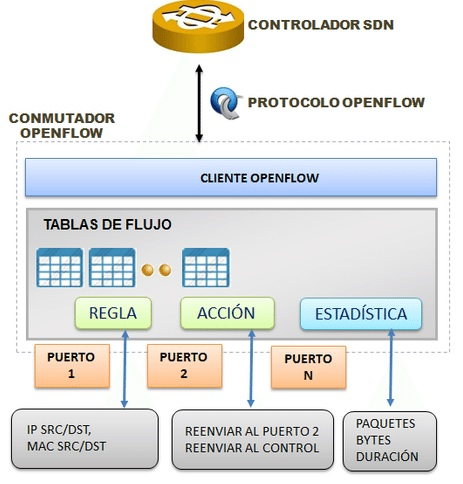
\includegraphics[width=0.7\linewidth]{imagenes/flujosOpenflow}
	\caption{Reglas de flujo en un Switch OpenFlow. Fuente: https://www.researchgate.net/figure/Figura-18-Estructura-y-componentes-de-un-conmutador-OpenFlow-Los-conmutadores-OpenFlow\_fig1\_312187600}
	\label{fig:flujosopenflow}
\end{figure}

\clearpage

En la figura \ref{fig:flujosopenflow} se puede ver la estructura de un \textit{switch} OpenFlow, así como la estructura interna de la tabla de flujos.

Cada vez que un \textit{switch} OpenFlow recibe un paquete, realiza un proceso de \textit{Matching}, es decir, comprueba si el paquete que ha recibido cumple algún selector de su tabla de flujos. Si algún selector coincide con dicho paquete, se reenvía según el tratamiento asociado a dicho selector.

En caso contrario, si dicho paquete no coincide con ninguna entrada de la tabla de flujos, se reenviara por un puerto por defecto, en función de la configuración del propio dispositivo.


\section{NFV}
\label{sec:nfv}

NFV (\textit{Network Function Virtualization}) es un paradigma que engloba a las redes de telecomunicación, más concretamente a su infraestructura. Su principal premisa es la de desacoplar las funciones de red de dispositivos \textit{hardware} y
 trasladarlas a servidores virtuales. Con ello se consigue tener múltiples funciones virtualizadas en un único servidor.

Las redes de telecomunicación actuales tienen ciertos problemas que NFV pretende resolver, como son:

\begin{itemize}
	\item Altos costes y restricciones físicas de fabricación.
	\item Complejidad \textit{hardware} en las soluciones del fabricante.
	\item Ciclo de vida corto de los dispositivos \textit{hardware}.
\end{itemize}

Todos estos problemas o desventajas han desembocado en la adopción de NFV como un estándar para agilizar, facilitar y escalar las infraestructuras de red, así como disminuir costes.

NFV reduce la dependencia de dispositivos \textit{hardware} dedicados. También mejora la escalabilidad y el uso de recursos, ya que una máquina de red puede ser replicada de forma más fácil que un dispositivo físico.

NFV tiene una serie de ventajas importantes que lo convierte en un alternativa óptima:

\begin{itemize}
	\item \textbf{Simplificar la implantación de elementos de red:} Las soluciones de red NFV son flexibles, genéricas y fáciles de implantar, lo que implica que el proceso de actualización es también más rápido y sencillo.
	
	\item \textbf{Mayor escalabilidad de la red:} Gracias a la naturaleza \textit{software} de las funciones virtualizadas, es mucho más fácil escalar los componentes de la red que si se trataran de dispositivos físicos.
	
	\item \textbf{Independencia respecto a los fabricantes de dispositivos:} Debido a que las funciones virtualizadas son desarrolladas mediante \textit{software}, se pierde la dependencia respecto a las particularidades de cada dispositivo, como su sistema operativo o su sintáxis de configuración y gestión, entre otros.
\end{itemize}

\subsection{Arquitectura NFV}
\label{subsec:nfvarq}

\begin{figure}[!ht]
	\centering
	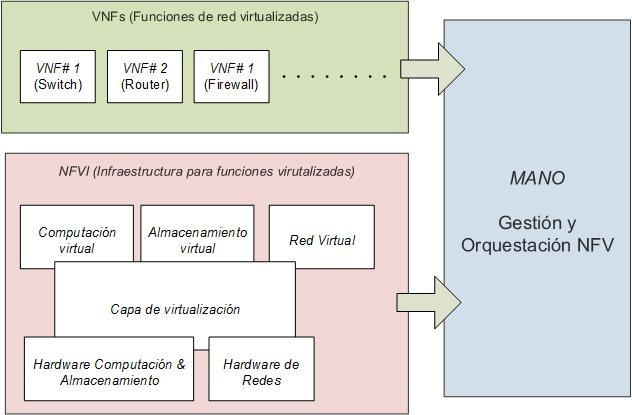
\includegraphics[width=0.75\linewidth]{imagenes/arquitectura_nfv}
	\caption{Arquitectura NFV Fuente: https://es.wikipedia.org/wiki/Virtualización\_de\_funciones\_de\_red}
	\label{fig:arquitecturanfv}
\end{figure}


\cleardoublepage